\section{1174042 Faisal Najib Abdullah}
\subsection{Teori}
\begin{enumerate}
\item Definisi, sejarah, dan perkembangan kecerdasan buatan.
\subitem Definisi kecerdasan buatan adalah suatu pengetahuan yang dapat membuat komputer untuk meniru kecerdasan manusia yang berhubungan dengan penangkapan, pemodelan, dan penyimpanan kecerdasan manusia dalam sebuah sistem teknologi. Contohnya yaitu melakukan analisa penalaran untuk mengambil suatu kesimpulan atau penerjemahan atau keputusan dari satu bahasa satu ke bahasa lain.
\subitem Sejarah dan perkembangan kecerdasan buatan terjadi pada musim panas tahun 1956 tercatat adanya seminar mengenai AI di Darmouth College. Seminar pada waktu itu dihadiri oleh sejumlah pakar komputer dan membahas potensi komputer dalam meniru kepandaian manusia. Akan tetapi perkembangan yang sering terjadi semenjak diciptakannya LISP, yaitu bahasa kecerdasan buatan yang dibuat tahun 1960 oleh John McCarthy. Istilah pada kecerdasan buatan atau Artificial Intelligence diambil dari Marvin Minsky dari MIT. Dia menulis karya ilmiah berjudul Step towards Artificial Intelligence, The Institute of radio Engineers Proceedings 49, January 1961\cite{baraja2008kecerdasan}. 
\item  Definisi supervised learning, klasifikasi, regresi, dan unsupervised learning. Data set, training set dan testing set. 
\subitem Supervised learning merupakan sebuah pendekatan dimana sudah terdapat data yang dilatih, dan terdapat variable yang ditargetkan sehingga tujuan dari pendekatan ini adalah mengkelompokan suatu data ke data yang sudah ada. Sedangkan unsupervised learning tidak memiliki data latih, sehingga dari data yang ada, kita mengelompokan data tersebut menjadi 2 bagian atau 3 bagian dan seterusnya.
\subitem Klasifikasi adalah salah satu topik utama dalam data mining atau machine learning. Klasifikasi yaitu suatu pengelompokan data dimana data yang digunakan tersebut mempunyai kelas label atau target.
\subitem Regresi adalah Supervised learning tidak hanya mempelajari classifier, tetapi juga mempelajari fungsi yang dapat memprediksi suatu nilai numerik. Contoh, ketika diberi foto seseorang, kita ingin memprediksi umur, tinggi, dan berat orang yang ada pada foto tersebut.
\subitem Data set adalah cabang aplikasi dari Artificial Intelligence/Kecerdasan Buatan yang fokus pada pengembangan sebuah sistem yang mampu belajar sendiri tanpa harus berulang kali di program oleh manusia.
\subitem Training set yaitu jika pasangan objek, dan kelas yang menunjuk pada objek tersebut adalah suatu contoh yang telah diberi label akan menghasilkan suatu algoritma pembelajaran.
\subitem Testing set digunakan untuk mengukur sejauh mana classifier berhasil melakukan klasifikasi dengan benar\cite{zhu2009introduction}.
\end{enumerate}

\subsection{Instalasi}
\subsubsection{Instalasi Library Scikit dari Pycharm}
Masuk pada menu settings terus pilih Project Interpreter kemudian tambah library lalu cari dan install scikit
\begin{figure}[ht]
\centering
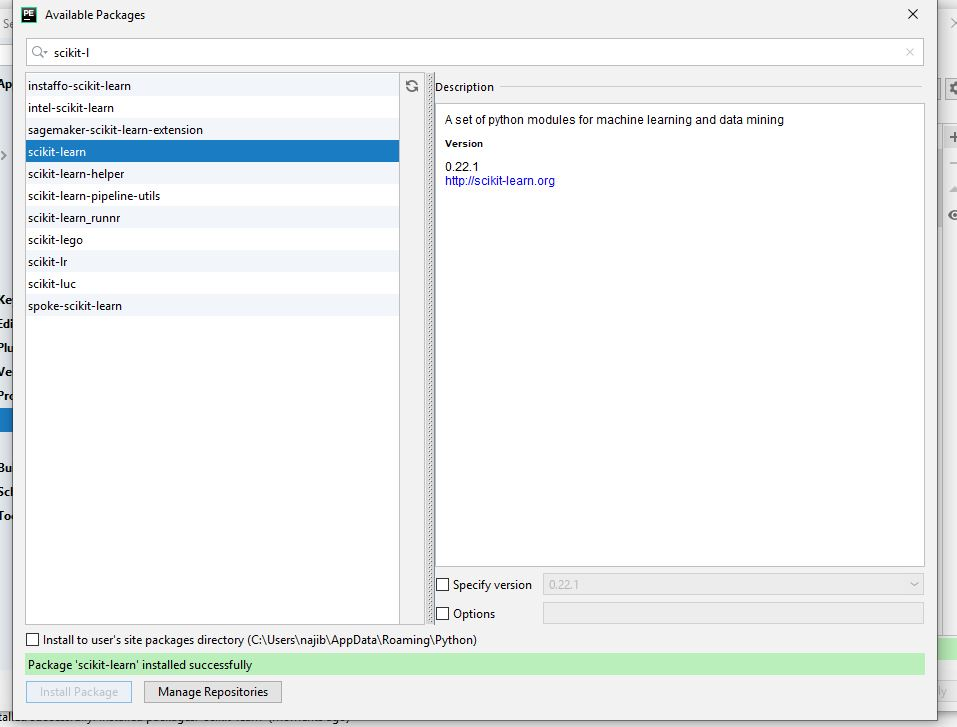
\includegraphics[scale=0.5]{figures/1174042/chapter1/2.jpg}
\caption{Installasi}
\label{contoh}
\end{figure}

Mencoba Library
\lstinputlisting{src/1174042/chapter1/2,1.py}

\subsubsection{Mencoba Loading an example Dataset}
\lstinputlisting{src/1174042/chapter1/2,2.py}
\begin{figure}[ht]
\centering
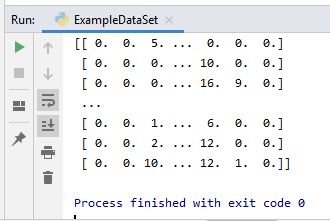
\includegraphics[scale=0.5]{figures/1174042/chapter1/3.jpg}
\caption{Mencoba Loading an example Dataset}
\label{contoh}
\end{figure}

\subsubsection{Learning and Predicting}
\lstinputlisting{src/1174042/chapter1/2,3.py}
\begin{figure}[ht]
\centering
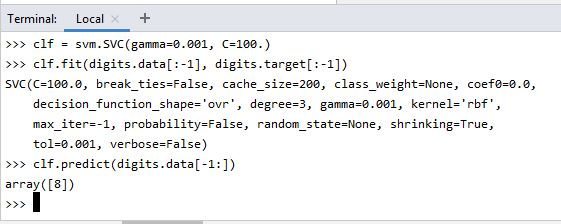
\includegraphics[scale=0.5]{figures/1174042/chapter1/2,3.jpg}
\caption{Learning and Predicting}
\label{contoh}
\end{figure}

\subsubsection{Model Presistence}
\lstinputlisting{src/1174042/chapter1/2,4.py}
\begin{figure}[ht]
\centering
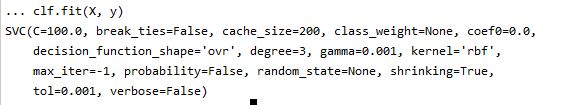
\includegraphics[scale=0.5]{figures/1174042/chapter1/2,4.jpg}
\caption{Model Presistence}
\label{contoh}
\end{figure}

\begin{figure}[ht]
\centering
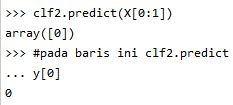
\includegraphics[scale=0.5]{figures/1174042/chapter1/2,4,1.jpg}
\caption{Model Presistence}
\label{contoh}
\end{figure}

\begin{figure}[ht]
\centering
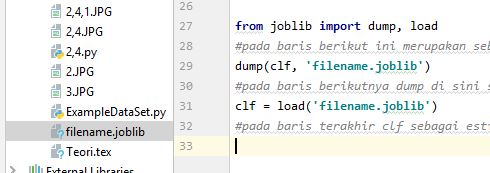
\includegraphics[scale=0.5]{figures/1174042/chapter1/2,4,2.jpg}
\caption{Model Presistence}
\label{contoh}
\end{figure}

\subsubsection{Conventions}
\lstinputlisting{src/1174042/chapter1/2,5.py}


\subsection{Penanganan eror}
\subsubsection{ScreenShoot Eror}
\begin{figure}[ht]
\centering
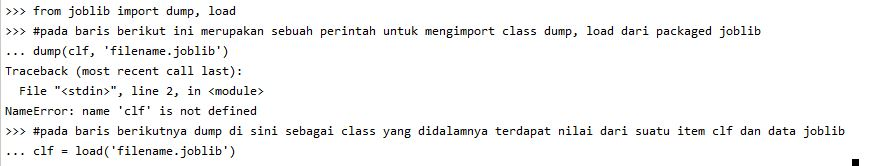
\includegraphics[scale=0.5]{figures/1174042/chapter1/3,1.jpg}
\caption{Error}
\label{contoh}
\end{figure}

\subsubsection{Tuliskan Kode Eror dan Jenis Erornya}
\begin{verbatim}
File "<stdin>", line 2, in <module>
NameError: name 'clf' is not defined
\end{verbatim}


\subsubsection{Solusi Pemecahan Masalah Error}
Ini karna kode di jalankan perbaris perbaris, jika kode dijanlankan bersamaan makan kode berjan sesuai prosedur.

\subsection{Plagiat}
\begin{figure}[ht]
\centering
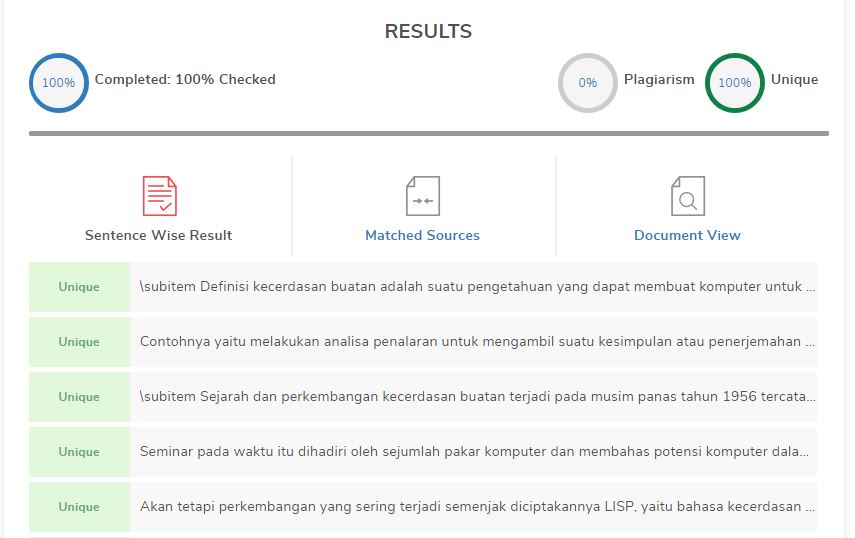
\includegraphics[scale=0.5]{figures/1174042/chapter1/5.jpg}
\caption{Error}
\label{contoh}
\end{figure}




\subsection{Link}
\href{https://youtu.be/oxm5CEsrsdY}{Youtube}